\documentclass[hidelinks, 12pt]{report}
\usepackage{graphicx}
\usepackage{marginnote}
\usepackage{amsmath}
\usepackage{amssymb}
\usepackage{geometry}
\usepackage[document]{ragged2e}
\usepackage[utf8]{inputenc}
\usepackage[english]{babel}
\usepackage{fancyhdr}
\usepackage{float}
%\usepackage{floatrow}
\usepackage{caption}
%\usepackage{calc}
\usepackage{chngcntr}
\usepackage[caption = false]{subfig}
\usepackage[subfigure]{tocloft}
\newlength{\mylen}
\usepackage[font=footnotesize,labelfont=bf]{caption}
%\usepackage{times}
\usepackage[table]{xcolor}
\usepackage[intoc]{nomencl}
\usepackage{setspace}
\usepackage{tocloft}

%\usepackage{nomencl}
%\let\abbrev\nomenclature
%\makenomenclature 
%\newcommand{\Abkuerzung}{
%\printnomenclature
%\newpage
%}


\usepackage{array}
\usepackage{hyperref}
\hypersetup{
    colorlinks=true,
    linkcolor=blue,
    filecolor=green,      
    urlcolor=cyan,
    citecolor=magenta,
}
\urlstyle{same}
\usepackage{bookmark}
\renewcommand{\cftfigpresnum}{\figurename\enspace}
\renewcommand{\cftfigaftersnum}{:}
\settowidth{\mylen}{\cftfigaftersnum\cftfigpresnum}
\addtolength{\cftfignumwidth}{\mylen}
\counterwithin{figure}{section}

\renewcommand{\cfttabpresnum}{\tablename\enspace}
\renewcommand{\cfttabaftersnum}{:}
\settowidth{\mylen}{\cfttabaftersnum\cftfigpresnum}
\addtolength{\cfttabnumwidth}{\mylen}
\counterwithin{table}{section}

\renewcommand{\labelenumi}{(\roman{enumi})}

\geometry{margin=1in}

\usepackage{titlesec}
\titleformat{\chapter}[display]
{\normalfont %
    \Huge % %change this size to your needs for the first line
    \bfseries}{\chaptertitlename\ \thechapter}{20pt}{%
    \huge} %change this size to your needs for the second line
 


\fancyhf{}
\fancyhead[LE,LO]{\footnotesize{}}
\fancyhead[RE,RO]{\footnotesize{Communications and Signals Design for Wireless Power Transmission}}
\fancyfoot[LE,LO]{\footnotesize{Govt. Model Engineering College}}
\fancyfoot[RE,RO]{\footnotesize\thepage}
\renewcommand{\headrulewidth}{1pt}
\renewcommand{\footrulewidth}{1pt}
%\renewcommand{\familydefault}{\rmdefault}
\newcommand{\Rnum}[1]{\uppercase\expandafter{\romannumeral#1}}
\newcommand{\rnum}[1]{\romannumeral#1\relax}
%\setcounter{secnumdepth}{4}
%\setcounter{tocdepth}{4}

\begin{document}
\pagenumbering{none}
\centering
\section*{\centering{Bonafide Certificate}}
\vspace{1cm}

\includegraphics[height=3cm,width=3cm]{logo}

\begin{center}
MODEL ENGINEERING COLLEGE\\
\vspace{0.5cm}
THRIKKAKARA, KOCHI-21\\
\vspace{0.5cm}
DEPARTMENT OF ELECTRONICS AND COMMUNICATION \\
\vspace{0.5cm}
APJ ABDUL KALAM TECHNOLOGICAL UNIVERSITY \\
\vspace{1cm}
\textit{Bonafide Certificate}
\\This is to Certify that the Seminar Report entitled\\
\vspace{0.5cm}
\textbf{Communications and Signals Design for Wireless Power Transmission} 
\\
\vspace{0.5cm}
Submitted by\\
\vspace{0.2cm}
M.G. Krishnan\\
\vspace{0.2cm}
is a bonafide account of his work done under our supervision. \\
\end{center}

\vspace{2cm}
\begin{minipage}[t]{10cm}
\flushleft \textbf{Seminar Co-ordinator}\\
Prof. Sunith C.K.\\
Assistant Professor\\
Dept. of Electronics and\\
Communication Engineering
\end{minipage}
\vspace{2cm}
\begin{minipage}[t]{5cm}
\flushleft \textbf{Seminar Guide}\\
Prof. Arun C.R.\\
Assistant Professor\\
Dept. of Electronics and\\
Communication Engineering
\end{minipage}
%\begin{minipage}[t]{5cm}
%\flushleft Head of Department\\
%Mr. Pradeep M\\
%Associate Professor\\
%\end{minipage}

%\addcontentsline{toc}{chapter}{Abstract}
\chapter*{Abstract}
\justify
\textit{
Radiative wireless power transfer (WPT) is a promising technology to provide cost-effective and real-time power supplies to wireless devices. Although radiative WPT shares many similar characteristics with the extensively studied wireless information transfer or communication, they also differ significantly in terms of design objectives, transmitter/receiver architectures and hardware constraints, etc. An overview on the various WPT technologies, the historical development of the radiative WPT technology and the main challenges in designing contemporary radiative WPT systems is given. The state-of-the-art communication and signal processing techniques that can be applied to tackle these challenges are also discussed. Topics discussed include energy harvester modeling, energy beamforming for WPT, channel acquisition, power region characterization in multi-user WPT, waveform design with linear and non-linear energy receiver model, safety and health issues of WPT, massive MIMO (multiple-input multiple-output) and millimeter wave (mmWave) enabled WPT, wireless charging control, and wireless power and communication systems codesign. Directions that are promising for future research are also discussed.}\\

\textit{\textbf{keyword}}- 
Wireless power transfer, energy beamforming, channel estimation and feedback, non-linear energy harvesting model, waveform design.
%\end{keyword}
%\sep%

\pagebreak
\setcounter{page}{1}
\pagenumbering{roman}
\justify
%\onehalfspacing
\begin{spacing}{0.8}
\renewcommand{\contentsname}{Table of Contents}
\pdfbookmark{\contentsname}{Table of Contents}
\tableofcontents
\end{spacing}
\pagebreak
%line spacing
\addcontentsline{toc}{chapter}{List of Figures}
\listoffigures 
\pagebreak
\renewcommand{\nomname}{List of Abbreviations}
\addcontentsline{toc}{chapter}{List of Abbreviations}
\printnomenclature
\pagebreak
%\addcontentsline{toc}{chapter}{List of Tables}
%\listoftables
%\pagebreak

\section*{List of Abbreviations}
\begin{flushleft}
WPT -  Wireless Power Transfer\\ 
\vspace{0.5cm}
MIMO - Multiple Input Multiple Output\\
\vspace{0.5cm}
LoS - Line of Sight\\
\vspace{0.5cm}
SWIPT - Simultaneous Wireless Information and Power Transfer\\
\vspace{0.5cm}
ET - Energy Transmitter\\
\vspace{0.5cm}
ER - Energy Receiver\\
\vspace{0.5cm}
RF - Radio Frequency\\
\vspace{0.5cm}
CSI - Channel State Information\\
\vspace{0.5cm}
OFDM - Orthogonal Frequency Division Multiplexing\\
\end{flushleft}
\pagebreak

\addcontentsline{toc}{chapter}{Acknowledgement}
\section*{Acknowledgement}
\justify
\\On the recollection of so many great favors and blessings, I offer my sincere thanks to the Almighty, the Creator and Preserver.\\
%\vspace{1cm}

I express my heartfelt gratitude to \textbf{Prof. Dr. V P Devassia}, Principal, Govt. Model Engineering College, Thrikkakara for providing me with excellent library facilities. \\
I am thankful to my seminar coordinator \textbf{Mr. Sunith C. K.}, Assistant Professor, Department of Electronics and Communication Engineering, and \textbf{Mrs. Swapna P. P.}, Assistant Professor, Department of Electronics and Communication Engineering for the full-fledged support and guidance. I sincerely thank \textbf{Prof. Arun C.R.} , Assistant Professor of Department of Electronics and Communication Engineering, for his timely advice and motivating me to do everything in a better way.\\

Last but not the least I am thankful to one and all of the Department of Electronics and Communication Engineering and the whole library staff for their co-operation and active involvement. I also thank my colleagues for their support.
\hbox{} \newpage 
\pagenumbering{arabic} 
\pagestyle{fancy}
\chapter{Introduction}
\justify
All kinds of electronic devices consume some form of energy or the other for its functioning. Devices such as cell phones, cameras, and laptops are powered by batteries, which have limited energy storage capacity. These batteries need to be regularly replaced or recharged. With the increase in use of portable devices such as cell phones, the need for powering up them wirelessly has also increased. Wireless charging can eliminate the need of connecting wires, can prove to be cost effective in the long run, avoids massive battery disposal and can be used in hazardous conditions. The key enabler for wireless charging is the advancement of wireless power transfer (WPT) technology. WPT refers to the technology of delivering power from a source to destination without interconnecting wires. Various WPT technologies have been developed so far, including inductive coupling, magnetic resonant coupling, electromagnetic radiation, and laser power beaming, among others. Right from 1880s, WPT has been in research with Heinrich Hertz demonstrating the existence and propagation of electromagnetic waves in free sapce. Advancements in microwave technology gave WPT the required boost. The development of magnetron tubes for highpower microwave generations and more advanced parabolic antennas for highly directional radiations helped bring advancements to the technology. Significant advancements have been made in the field of Magnetic Resonant Coupling WPT and Inductive Coupling WPT. However, these technologies are limited with short range, lower efficiency at longer range, size of transmitters and receivers. Radiative WPT on the other hand, increased the range significantly, eliminates the need for Line of Sight transmission and enables use of Multiple Input Multiple Output (MIMO). Radiative WPT also allows high power transmissions and can be used in Standby Power Supply (SPS).  
\begin{figure}[H]
\centering
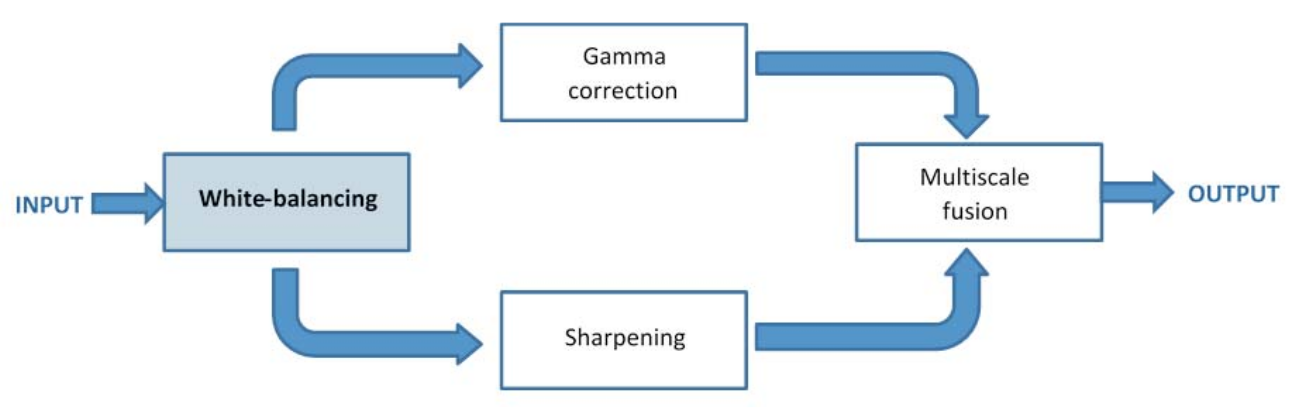
\includegraphics[width=15cm,height=5cm]{Block.png}
\caption[Method Overview]{Method Overview}
\label{Method Overview}
\end{figure}
\chapter{Background Knowledge and Previous Art}
\section{Light Propogation in Underwater Environment}
\justify
For an ideal transmission medium the received light is influenced mainly by the properties of the target objects and the camera lens characteristics. This is not the case underwater. First, the amount of light available under water, depends on several factors. The interaction between the sun light and the sea surface is affected by the time of the day (which influences the light incidence angle), and by the shape of
the interface between air and water (rough vs. calm sea). The diving location also directly impacts the available light, due to a location-specific color cast: deeper seas and oceans induce green and blue casts, tropical waters appear cyan, while protected reefs are characterized by high visibility. In addition to the variable amount of light available underwater, the density of particles that the light has to go through
is several hundreds of times denser in seawater than in normal atmosphere. As a consequence, sub-sea water absorbs gradually different wavelengths of light. Red, which corresponds to the longest wavelength, is the first to be absorbed (10-15 ft), followed by orange (20-25 ft), and yellow (35-45 ft). Pictures taken at 5 ft depth will have a noticeable loss of red. Further-more, the refractive index of water makes judging distances difficult. As a result, underwater objects can appear 25\% larger than they really are. The comprehensive studies have shown that the total irradiance incident on a generic point of the image plane has three main components in underwater mediums: direct component, forward scattering and back scattering. The direct component is the component of light reflected directly by the target object onto the image plane. At each image coordinate x the direct component is expressed as:
\begin{equation}
E_D(x)=J(x)e^{-\eta d(x)}=J(x)t(x)
\end{equation}
where $J(x)$ is the radiance of the object, $d(x)$ is the distance between the observer and the object, and $\eta$ is the attenuation coefficient. The exponential term $e^{−\eta d(x)}$ is also known as the transmission $t(x)$ through the underwater medium.\\
Besides the absorption, the floating particles existing in the underwater mediums also cause the deviation (scattering) of the incident rays of light. Forward-scattering results from a random deviation of a light ray on its way to the camera lens. It has been determined experimentally that its impact can be approximated by the convolution between the direct attenuated component, with a point spread function that depends on the distance between the image plane and the object. Back-scattering is due to the artificial light (e.g. flash) that hits the water particles, and is reflected back to the camera. Back-scattering acts like a glaring veil superimposed on the object. The influence of this component may be reduced significantly by simply changing the position and angle of the artificial light source so that most of the reflected particle light do not reach the camera. However, in many practical cases, back-scattering remains the principal source of contrast loss and color shifting in underwater images. Mathematically, it is often expressed as:
\begin{equation}
E_{BS}(x)=B_{\infty}(x)(1-e^{-\eta d(x)})
\end{equation}
where $B_{\infty}(x)$ is a color vector known as the \textit{back-scattered} light.\\
Ignoring the forward scattering component, the simplified underwater optical model thus becomes:
\begin{equation}
I(x)=J(x)e^{-\eta d(x)}+B_{\infty}(x)(1-e^{-\eta d(x)})
\end{equation}
This simplified underwater camera model is used to characterize the propagation of light in the atmosphere. It however does not reflect the fact that the attenuation coefficient strongly depends on the light wavelength, and thus the color, in underwater environments. Therefore, as discussed in the next section, a straightforward extension of outdoor dehazing approaches performs poorly at great depth, in presence of non-uniform artificial illumination and selective absorption of colors. It is also why this approach does not resort to an explicit inversion of the light propagation model.
\section{Related Works}
\justify
The existing underwater dehazing techniques can be grouped in several classes. 
\begin{itemize}
\item{Using specialized hardware - For instance, the divergent-beam underwater Lidar imaging (UWLI) system uses an optical/laser-sensing technique to capture turbid underwater images. Unfortunately, these complex acquisition systems are very expensive, and power consuming.}
\item{Polarization-based methods - These approaches use several images of the same scene captured with different degrees of polarization, as obtained by rotating a polarizing filter fixed to the camera. While being effective in recovering distant regions, the polarization techniques are not applicable to video acquisition, and are therefore of limited help when dealing with dynamic scenes.}
\item{Multiple images - A rough approximation of the scene model is created with huge amount of data. Since this additional information (images and depth approximation) is generally not available, these methods are impractical for common users.}
\item{Exploiting the similarities between light propagation in fog and under water - Several single image dehazing techniques have been introduced to restore images of outdoor foggy scenes. These dehazing techniques reconstruct the intrinsic brightness. Several works have shown that it can be used in heterogeneous lightning conditions and with heterogeneous extinction coefficient as long as the model parameters are estimated locally. However, the underwater imaging is even more challenging, due to the fact that the extinction resulting from scattering depends on the light wavelength, i.e. on the color component.}
\end{itemize}
Recently, several algorithms that specifically restore underwater images based on Dark Channel Prior (DCP), have been introduced. The DCP has initially been proposed for outdoor scenes dehazing. It assumes that the radiance of an object in a natural scene is small in at least one of the color component, and consequently defines regions of small transmission as the ones with large minimal value of colors. In the underwater context, many approaches were considered:
\begin{itemize}
\item{Segmenting foreground and background regions based on DCP, and uses this information to remove the haze and color variations based on color compensation.}
\item{Assuming that the predominant source of visual information under the water lies in the blue and green color channels. Their Underwater Dark Channel Prior (UDCP) has been shown to estimate better the transmission of underwater scenes than the conventional DCP.}
\item{Observations that the red component reciprocal increases with the distance to the camera introduced the Red Channel Prior to recover colors associated with short wavelengths in underwater.}
\item{Designing a hierarchical rank based method, using a set of features to find those image regions that are the most haze-opaque, thereby refining the back-scattered light estimation, which in turns improves the light transmission model inversion.}
\item{Employing color lines to estimate the ambient light and implement a variant of the DCP to estimate the transmission.}
\item{Bilateral filter is considered to remove highlighted regions before ambient light estimation, and another locally adaptive filter is considered to refine the transmission.}
\item{Extending colour lines to increase the resolution of its descattered and color-corrected output. This extension builds on super-resolution from transformed self-exemplars to derive two high-resolution (HR) images, respectively from the output derived in and from a denoised/descattered version of this output. A fusion-based strategy is then considered to blend those two intermediate HR images. This fusion aims at preserving the edges and detailed structures of the noisy HR image, while taking advantage of the reduced noise and scatter in the second HR image. It however does not impact the rendering of color obtained.}
\end{itemize}
\chapter{Underwater White Balance}
\justify
This image enhancement approach adopts a two step strategy, combining white balancing and image fusion, to improve underwater images without resorting to the explicit inversion of the optical model. Here, white balancing aims at compensating for the color cast caused by the selective absorption of colors with depth, while image fusion is considered to enhance the edges and details of the scene, to mitigate the loss of contrast resulting from back-scattering.\\ White-balancing aims at improving the image aspect, primarily by removing the undesired color castings due to various illumination or medium attenuation properties. In underwater, the perception of color is highly correlated with the depth, and an important problem is the green-bluish appearance that needs to be rectified. As the light penetrates the water, the attenuation process affects selectively the wavelength spectrum, thus affecting the intensity and the appearance of a colored surface. Since the scattering attenuates more the long wavelengths than the short ones, the color perception is affected as we go down in deeper water. In practice, the attenuation and the loss of color also depends on the total distance between the observer and the scene. Large spectrum of existing white balancing methods were considered, a number of solutions were identified that are both effective and suited to the problem.\\ The following are those approaches which played a major role the derivation of this novel approach proposed for underwater scenes.
\begin{itemize}
\item{Gray world algorithm assumes that the average reflectance in the scene is achromatic. Hence, the illuminant color distribution is simply estimated by averaging each channel independently.}
\item{The Max RGB assumes that the maximum response in each channel is caused by a white patch, and consequently estimates the color of the light source by employing the maximum response of the different color channels.}
\item{The ‘Shades-of-Grey’ method, Max-RGB and Gray-World are two instantiations of the Minkowski $p$-norm applied to the native pixels,  espectively with $p=\infty$ and $p=1$, and propose to extend the process to arbitrary $p$ values. The best results are obtained for $p=6$.}
\item{The Grey-Edge hypothesis further extends this Minkowski norm framework. It assumes the average edge difference in a scene to be achromatic, and computes the scene illumination color by applying the Minkowski p-norm on the derivative structure of image channels, and not on the zero-order pixel structure, as done in Shades of Grey. Despite of its computational simplicity, this approach has been shown to obtain comparable results than state-of-the-art color constancy methods, such as the recent method that relies on natural image statistics.}
\end{itemize}
\begin{figure}[H]
\centering
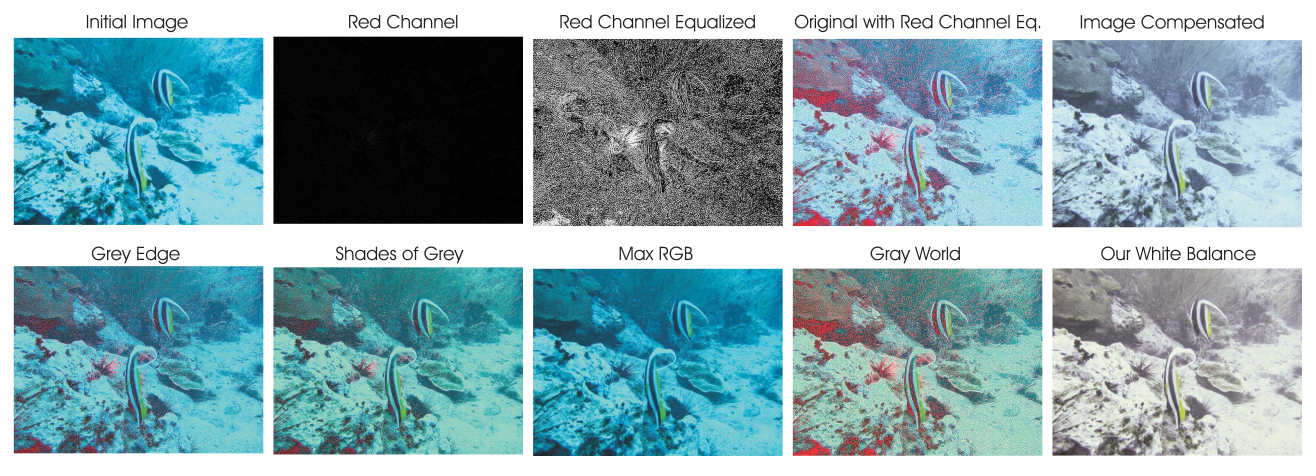
\includegraphics[width=15cm,height=5cm]{White.png}
\caption[Underwater White Balance]{Underwater White Balance}
\label{Underwater White Balance}
\end{figure}
When focusing on underwater scenes, the well-known Gray-World algorithm achieves good visual performance for reasonably distorted underwater scenes. However, a deeper investigation dealing with extremely deteriorated underwater scenes revealed that most traditional methods perform poorly. They fail to remove the color shift, and generally look bluish. The methods that best remove the bluish tone is the Grey World, but we observe that this method suffers from severe red artifacts. Those artifacts are due to a very small mean value for the red channel, leading to an overcompensation of this channel in locations where red is present (because Gray world devides each channel by its mean value).\\
To compensate for the loss of red channel, the following observations/principles were proposed:
\begin{itemize}
\item{The green channel is relatively well preserved under water, compared to the red and blue ones. Light with a long wavelength, i.e. the red light, is indeed lost first when traveling in clear water.}
\item{The green channel is the one that contains opponent color information compared to the red channel, and it is thus especially important to compensate for the stronger attenuation induced on red, compared to green. Therefore, to compensate the red attenuation, a fraction of the green channel is added to red. The information of the green channel alone allows better recovery of the entire color spectrum while maintaining a natural appearance of the background(water regions) than adding both a fraction of green and blue to the red.}
\item{The compensation should be proportional to the difference between the mean green and the mean red values because, under the Gray World assumption (all channels have the same mean value before attenuation), this difference reflects the disparity/unbalance between red and green attenuation.}
\item{To avoid saturation of the red channel during the Gray World step that follows the red loss compensation, the enhancement of red should primarily affect the pixels with small red channel values, and should not change pixels that already include a significant red component. In other words, the green channel information should not be transferred in regions where the information of the red channel is still significant. Thereby, the reddish appearance introduced by the Gray-World algorithm in the over-exposed regions should be avoided. Basically, the compensation of the red channel has to be performed only in those regions that are highly attenuated. This argument follows the statement, telling that if a pixel has a significant value for the three channels, this is because it lies in a location near the observer, or in an artificially illuminated area, and does not need to be restored.}
\end{itemize}
Mathematically, to account for the above observations, we propose to express the compensated red channel $I_{rc}$ at every pixel location $(x)$ as follows:
\begin{equation}
I_{rc}(x)=I_r(x)+\alpha.(\overline{I}_g-\overline{I}_r).(1-I_r(x)).I_g(x)
\end{equation}
where $I_r$, $I_g$ represent the red and green color channels of image $I$, each channel being in the interval $[0, 1]$, after normalization by the upper limit of their dynamic range, while $\overline{I}_r$ and $\overline{I}_g$ denote the mean value of $I_r$ and $I_g$. Each factor in the second term directly results from one of the above observations, and α denotes a constant parameter. In practice, our tests have revealed that a value of $\alpha=1$ is appropriate for various illumination conditions and acquisition settings.\\
To complete our discussion about the severe and color-dependent attenuation of light under water, it is worth noting the works, which reveal and exploit the fact that, in turbid waters or in places with high concentration of plankton, the blue channel may be significantly attenuated due to absorption by organic matter. To address those cases, when blue is strongly attenuated and the compensation of the red channel appears to be insufficient, we propose to also compensate for the blue channel attenuation, i.e. we compute the compensated blue channel $I_{bc}$ as:
\begin{equation}
I_{bc}(x)=I_b(x)+\alpha.(\overline{I}_g-\overline{I}_b).(1-I_b(x)).I_g(x)
\end{equation}
where $I_b$ , $I_g$ represent the blue and green color channels of image $I$, and $\alpha$ is also set to $1$. After the red (and optionally the blue) channel attenuation has been compensated, the conventional Gray-World assumption is done to estimate and compensate the illuminant color cast. This white-balancing approach reduces the quantization artifacts introduced by domain stretching (the red regions in the different outputs). The reddish appearance of high intensity regions is also well corrected since the red channel is better balanced.\\
Additionally, this white balancing strategy yields significant improvement in estimating transmission based on the well-known DCP. Estimating the transmission maps based on DCP, using the initial underwater images but also the processed versions with several well-known white balancing approaches (Gray Edge, Shades of Gray, Max RGB and Gray World) yields poor estimates. In contrast, by simply applying DCP on our white balanced
image version we obtain comparable and even better estimates than the specialized underwater techniques of UDCP, MDCP and BP.
\begin{figure}[H]
\centering
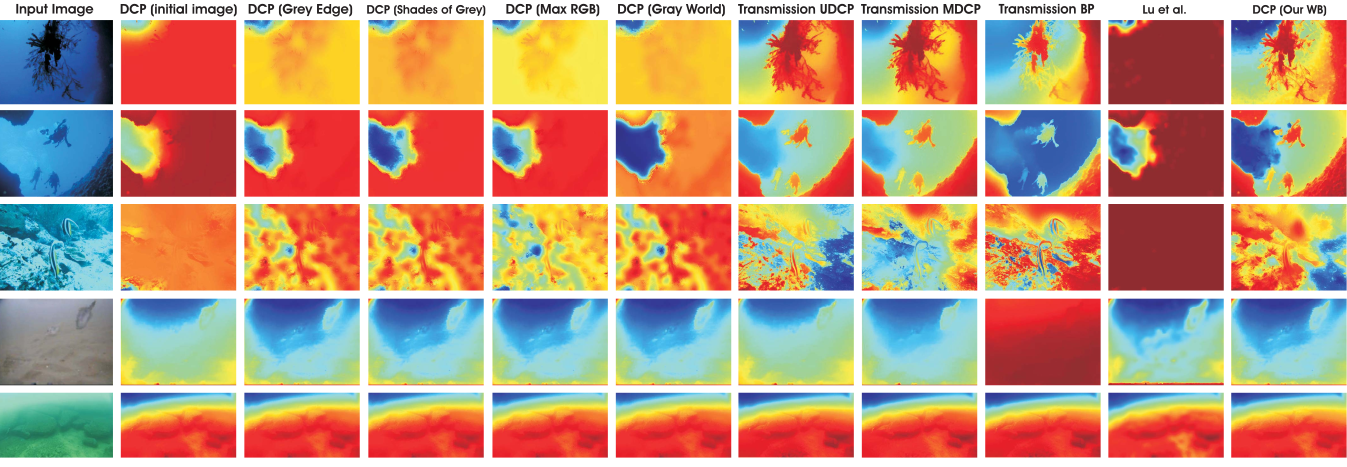
\includegraphics[width=15cm,height=5cm]{Transmission.png}
\caption[Underwater Transmission Estimation]{Underwater Transmission Estimation}
\label{Underwater Transmission Estimation}
\end{figure}

\chapter{Multi-Scale Fusion}
\justify
Image fusion has shown utility in several applications such as image compositing, multispectral video enhancement, defogging, and HDR imaging. Here, the aim is a simple and fast approach that is able to increase the scene visibility in a wide range of underwater videos and images. This framework builds on a set of inputs and weight maps derived from a single original image. A pair of inputs is introduced to respectively enhance the color contrast and the edge sharpness of the white-balanced image, and the weight maps are defined to preserve the qualities and reject the defaults of those inputs, i.e. to overcome the artifacts induced by the light propagation limitation in underwater medium.\\To derive the inputs from the original image, the CVPR algorithm did assume that the back-scattering component (due to the artificial light that hits the water particles and is then reflected back to the camera) has a reduced influence. This assumption is generally valid for underwater scenes decently illuminated by natural light, but fails in more challenging illumination scenarios. Alternative definition of inputs and weights are taken in order to deal with severley degraded scenes without relying on the optical model.\\ This underwater dehazing technique consists in three main steps: inputs derivation from the white balanced underwater image, weight maps definition, and multi-scale fusion of the inputs and weight maps.

\section{Inputs of the Fusion Process}
Since the color correction is critical in underwater, first the white balancing technique is applied to the original image. This step aims at enhancing the image appearance by discarding unwanted color casts caused by various illuminants. In water deeper than 30 ft, white balancing suffers from noticeable effects since the absorbed colors are difficult to be recovered. As a result, to obtain the \textbf{first} input, a gamma correction of the white balanced image version is performed. Gamma correction aims at correcting the global contrast and is relevant since, in general, white balanced underwater images tend to appear too bright. This correction increases the difference between darker/lighter regions at the cost of a loss of details in the under-/over-exposed regions.\\ To compensate for this loss, a \textbf{second} input is derived that corresponds to a sharpened version of the white balanced image. Therefore, the unsharp masking principle is followed in the sense that a blurred or unsharp (here Gaussian filtered) version of the image is blended with the image to sharpen. The typical formula for unsharp masking defines the sharpened image $S$ as $S=I+\beta(I-G*I)$, where $I$ is the image to sharpen (in our case the white balanced image), $G∗I$ denotes the Gaussian filtered version of $I$, and $\beta$ is a parameter. In practice, the selection of $\beta$ is not trivial. A small $\beta$ fails to sharpen $I$, but a too large $\beta$ results in over-saturated regions, with brighter highlights and darker shadows. To circumvent this problem, the sharpened image $S$ is defined as follows:
\begin{equation}
S=(I+N(I-G*I))/2
\end{equation}
with $N{.}$ denoting the linear normalization operator, also named histogram stretching in the literature. This operator shifts and scales all the color pixel intensities of an image with a unique shifting and scaling factor defined so that the set of transformed pixel values cover the entire available dynamic range.The sharpening method defined is referred to as normalized unsharp masking process in the following. It has the advantage to not require any parameter tuning, and appears to be effective in terms of sharpening. 
\begin{figure}[H]
\centering
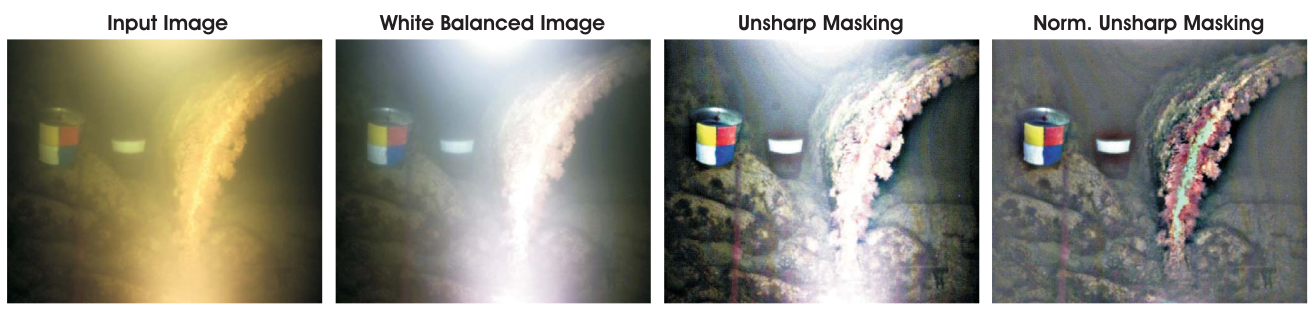
\includegraphics[width=15cm,height=3.5cm]{NUM.png}
\caption[Comparison between traditional Unsharp Masking and normalized Unharp Masking]{Comparison between traditional unsharp masking and normalized Unharp Masking}
\label{Comparison between traditional Unsharp Masking and normalized Unharp Masking}
\end{figure}
This second input primarily helps in reducing the degradation caused by scattering. Since the difference between white balanced image and its Gaussian filtered version is a highpass signal that approximates the opposite of Laplacian, this operation has the inconvenient to magnify the high-frequency noise, thereby generating undesired artifacts in the second input. The multi-scale fusion strategy described in the next section will be in charge of minimizing the transfer of those artifacts to the final blended image.

\section{Weights of the Fusion Process}
The weight maps are used during blending in such a way that pixels with a high weight value are more represented in the final image. They are thus defined based on a number of local image quality or saliency metrics.
\begin{itemize}
\item{\textbf{\textit{Laplacian contrast weight}} ($W_L$) estimates the global contrast by computing the absolute value of a Laplacian filter applied on each input luminance channel. This straightforward indicator was used in different applications such as tone mapping and extending depth of field since it assigns high values to edges and texture. For the underwater dehazing task, however, this weight is not sufficient to recover the contrast, mainly because it can not distinguish much between a ramp and flat regions. So additional and complementary constrast assessment metric is introduced.}
\item{\textbf{\textit{Saliency weight}} ($W_S$) aims at emphasizing the salient objects that lose their prominence in the underwater scene. To measure the saliency level, a saliency estimator is employed. This computationally efficient algorithm has been inspired by the biological concept of center-surround contrast. However, the saliency map tends to favor highlighted areas (regions with high luminance values). To overcome this limitation, an additional weight map based on the observation that saturation decreases in the highlighted regions is introduced.}
\item{\textbf{\textit{Saturation weight}} ($W_{Sat}$) enables the fusion algorithm to adapt to chromatic information by advantaging highly saturated regions. This weight map is simply computed (for each input $I_k$) as the deviation (for every pixel location) between the $R_k$, $G_k$ and $B_k$ color channels and the luminance $L_k$ of the $k^{th}$ input:
\begin{equation}
W_{sat}=\sqrt{(1/3)[(R_k-L_k)^2+(G_k-L_k)^2+(B_k-L_k)^2]}
\end{equation}
}
\end{itemize}
\begin{figure}[H]
\centering
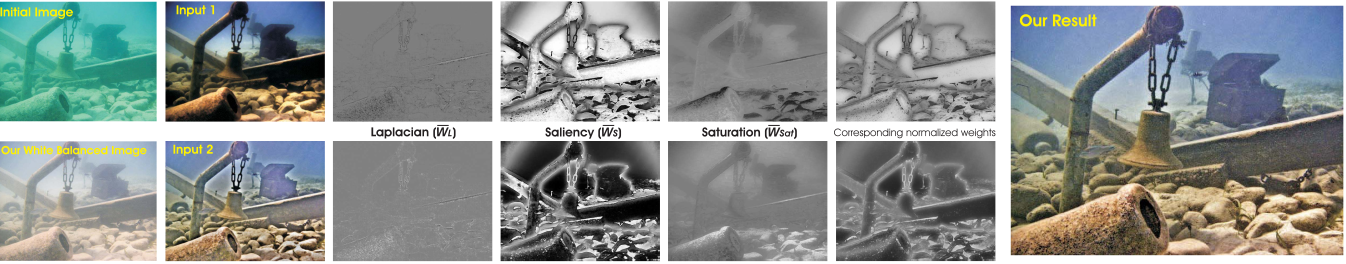
\includegraphics[width=15cm,height=3cm]{Weight.png}
\caption[Weight Maps]{Weight Maps}
\label{Weight Maps}
\end{figure}
In practice, for each input, the three weight maps are merged in a single weight map as follows. For each input $k$, an aggregated weight map $W_k$ is first obtained by summing up the three $W_L$ , $W_S$ , and $W_{Sat}$ weight maps. The $K$ aggregated maps are then normalized on a pixel-per-pixel basis, by dividing the weight of each pixel in each map by the sum of the weights of the same pixel over all maps. Formally, the
normalized weight maps $\overline{W}_k$ are computed for each input as:
\begin{equation}
\overline{W}_{k}=(W_k+\delta)/(\sum_{k=1}^{K}W_k + K.\delta)
\end{equation}
with $\delta$ denoting a small regularization term that ensures that each input contributes to the output. $\delta$ is set to 0.1 in the rest of the paper. The normalized weights of corresponding weights are shown. These three weight maps are used. The exposedness weight map tends to amplify some artifacts, such as ramp edges of our second input, and to reduce the benefit derived from the gamma corrected image in terms of image contrast. Originally, in an exposure fusion context, the exposedness weight map had been introduced to reduce the weight of pixels that are under- or over-exposed. Hence, this weight map assigns large (small) weight to input pixels that are close to (far from) the middle of the image dynamic range. Here since the gamma corrected input tends to exploit the whole dynamic range, the use of the exposedness weight map tends to penalize it in favor of the sharpened image, thereby inducing some sharpening artifacts and missing some contrast enhancements.

\section{Naive Fusion Process}
Given the normalized weight maps, the reconstructed image $R(x)$ could typically be obtained by fusing the defined inputs with the weight measures at every pixel location $(x)$:
\begin{equation}
R(x)=\sum_{k=1}^{K}\overline{W}_k(x)I_k(x)
\end{equation}
where $I_k$ denotes the input ($k$ is the index of the inputs $K=2$ in our case) that is weighted by the normalized weight maps $\overline{W}_k$. In practice, the naive approach introduces undesirable halos. A common solution to overcome this limitation is to employ multi-scale linear, or non-linear filters.

\section{Multi-Scale Fusion Process}
The multi-scale decomposition is based on Laplacian pyramid. The pyramid representation decomposes an image into a sum of bandpass images. In practice, each level of the pyramid does filter the input image using a low-pass Gaussian kernel $G$, and decimates the filtered image by a factor of 2 in both directions. It then subtracts from the input an up-sampled version of the low-pass image, thereby approximating the (inverse of the) Laplacian, and uses the decimated low-pass image as the input for the subsequent level of the pyramid. Formally, using $G_l$ to denote a sequence of $l$ low-pass filtering and decimation, followed by $l$ up-sampling operations, we define the $N$ levels $L_l$ of the pyramid as follows:
\begin{equation}
\begin{split}
I(x) & = I(x)-G_1[I(x)]+G_1[I(x)] \triangleq L_1[I(x)]+G_1[I(x)]\\
& = L_1[I(x)]+G_1[I(x)]-G_2[I(x)]+G_2[I(x)]\\
& = L_1[I(x)]+L_2[I(x)]+G_2[I(x)]\\
& = ...\\
& = \sum_{l=1}^{N}L_l[I(x)]
\end{split}
\end{equation}
In this equation, $L_l$ and $G_l$ represent the $l^{th}$ level of the Laplacian and Gaussian pyramid, respectively. To write the equation, all those images have been up-sampled to the original image dimension. However, in an efficient implementation, each level $l$ of the pyramid is manipulated at native subsampled resolution. Following the traditional multi-scale fusion strategy, each source input $I_k$ is decomposed into a Laplacian pyramid while the normalized weight maps $\overline{W}_k$ are decomposed using a Gaussian pyramid. Both pyramids have the same number of levels, and the mixing of the Laplacian inputs with the Gaussian normalized weights is performed independently at each level $l$:
\begin{equation}
R_l(x)=\sum_{k=1}^{K}G_l[\overline{W}_k(x)]L_1[I_k(x)]
\end{equation}
where $l$ denotes the pyramid levels and $k$ refers to the number of input images. In practice, the number of levels $N$ depends on the image size, and has a direct impact on the visual quality of the blended image. The dehazed output is obtained by summing the fused contribution of all levels, after appropriate upsampling.
\begin{figure}[H]
\centering
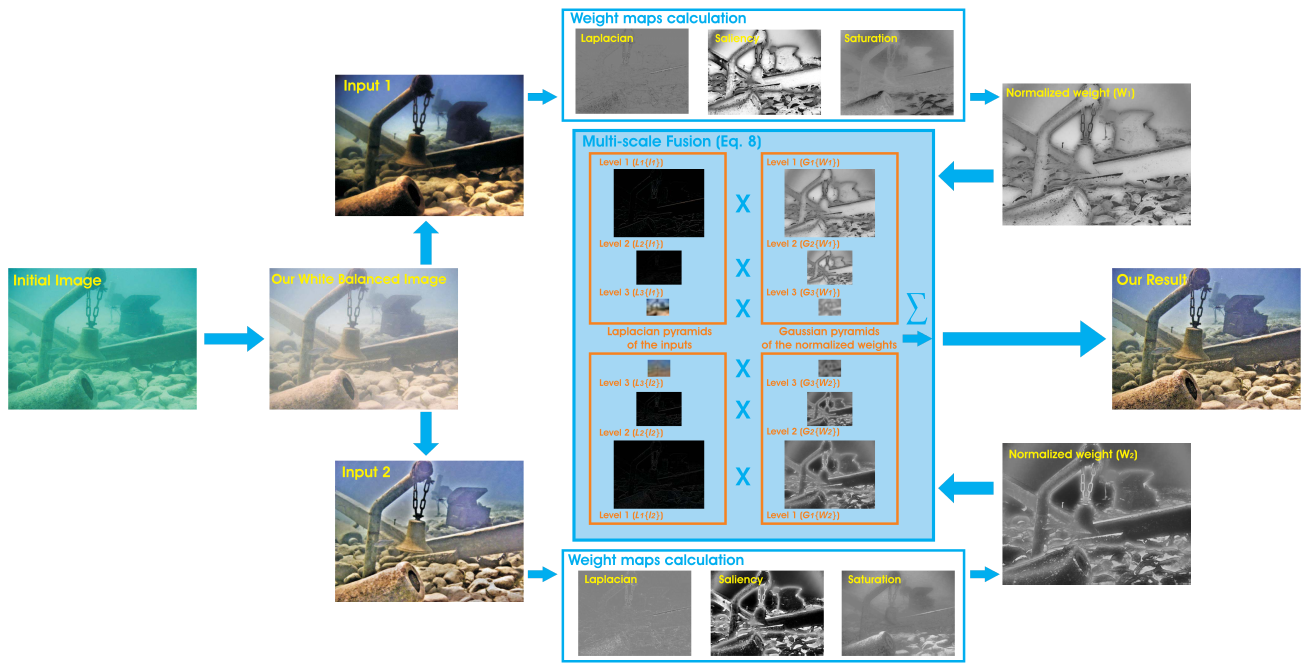
\includegraphics[width=16cm,height=8cm]{Dehaze.png}
\caption[Overview of Dehazing Schemes]{Overview of Dehazing Schemes}
\label{Overview of Dehazing Schemes}
\end{figure}
By independently employing a fusion process at every scale level, the potential artifacts due to the sharp transitions of the weight maps are minimized. Multi-scale fusion is motivated by the human visual system, which is very sensitive to sharp transitions appearing in smooth image patterns, while being much less sensitive to variations/artifacts occurring on edges and textures (masking phenomenon). This single- scale approximation should definitely be encouraged when complexity is an issue, since it also turns the multiresolution process into a spatially localized procedure.

\chapter{Results and Discussion}
This dehazing technique is compared with the existing specialized underwater restoration/enhancement techniques and the utility of this approach for applications such as segmentation and keypoint matching is proved.
\section{Video Dehazing}
The proposed strategy was tested for real underwater image and videos taken from different available amateur and professional photographer collections, captured using various cameras and setups. Processing only 8-bit data format makes this validation relevant for common
low-end cameras. Interestingly, this fusion-based algorithm has the advantage to employ only a reduced set of parameters that can be automatically set. Specifically, the white balancing process relies on the single parameter $\alpha$, which is set to 1 in all our experiments. For the multi-scale fusion, the number of decomposition levels depends on the image size, and is defined so that the size of the smallest resolution reaches a few tenth of pixels.
\begin{figure}[H]
\centering
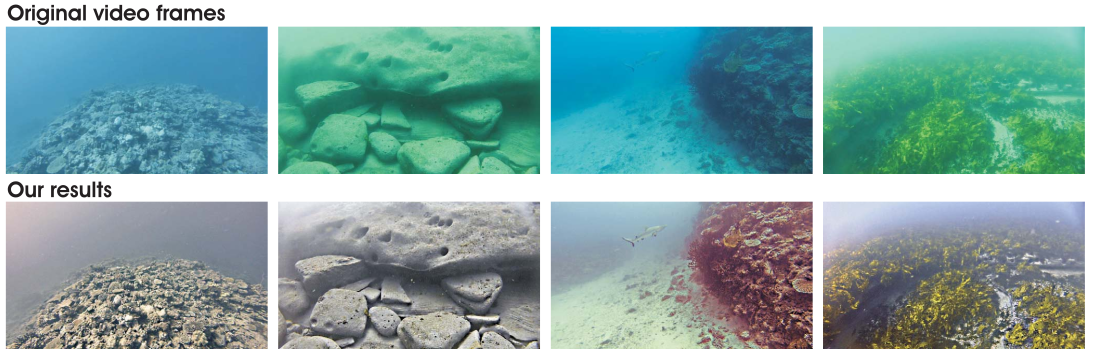
\includegraphics[width=15cm,height=5cm]{Video.png}
\caption[Underwater Video Dehazing]{Underwater Video Dehazing}
\label{Underwater Video Dehazing}
\end{figure}
This approach generally results in good perceptual quality, with significant enhancement of the global contrast, the color, and the image structure details. The main limitations are related to the fact that: (i) color can not always be fully restored, and (ii) some haze is maintained, especially in the scene regions that are far from the camera. Those limitations are however limited, especially when compared to previous works.
\section{Applications}
\subsection{Segmentation}
Segmentation aims at dividing images into disjoint and homogeneous regions with respect to some characteristics (e.g. texture, color). In this work, we employ the GAC++ segmentation algorithm, which corresponds to a seminal geodesic active contours method (variational PDE). The segmentation result is more consistent when segmentation is applied to images that have been processed by this approach.
\begin{figure}[H]
\centering
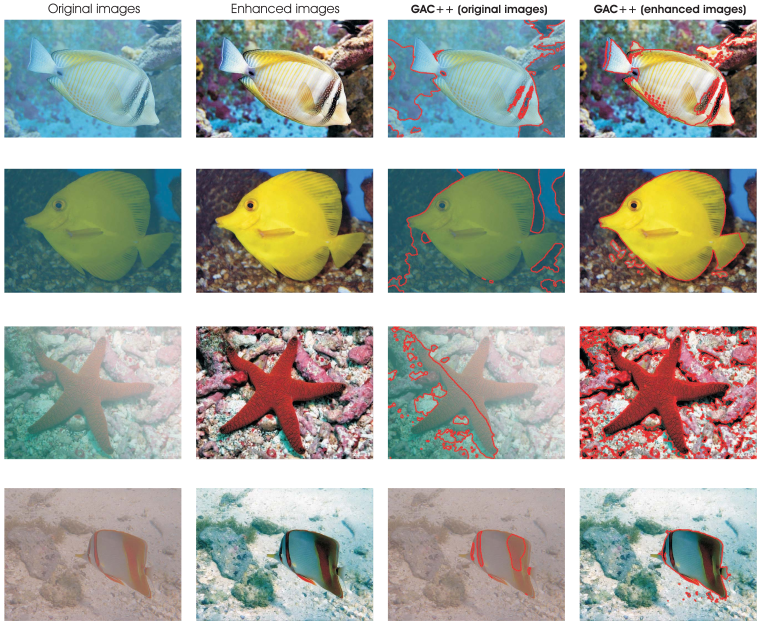
\includegraphics[width=15cm,height=13cm]{Segment.png}
\caption[Image Segmentation]{Image Segmentation}
\label{Image Segmentation}
\end{figure}
\subsection{Local Feature-point Matching}
Local feature points matching is a fundamental task of many computer vision applications. The SIFT operator is employed to compute keypoints, and compare the keypoint computation and matching processes for a pair of underwater images, with the one computed for the corresponding pair of images enhanced by this method. The original implementation of SIFT is applied exactly in the same way in both cases. The promising achievements presented demonstrates that, by enhancing the global contrast and the local features in underwater images, our method significantly increases the number of matched pairs of keypoints.
\begin{figure}[H]
\centering
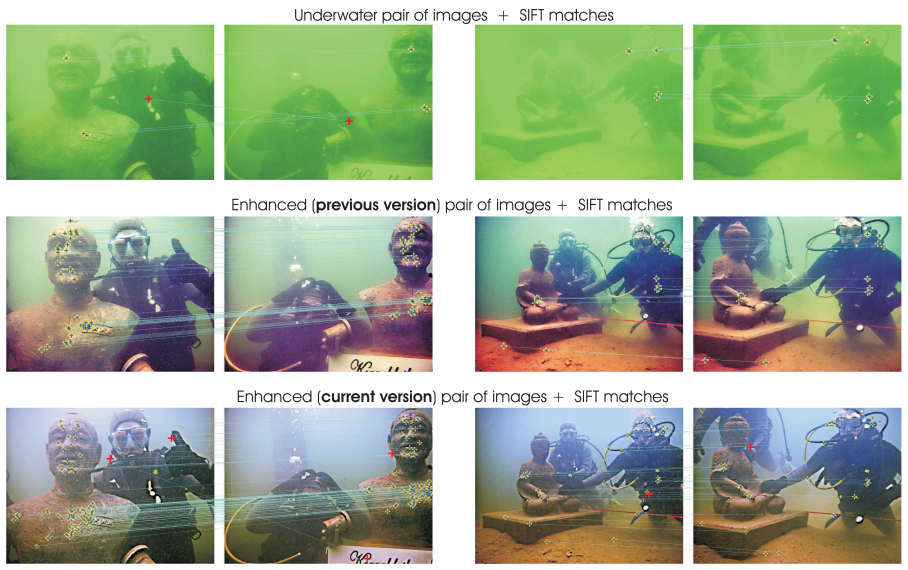
\includegraphics[width=15cm,height=9cm]{Feature.png}
\caption[Local Feature-point Matching]{Local Feature-point Matching}
\label{Local Feature-point Matching}
\end{figure}

\chapter{Conclusion}
This Single image Fusion process an alternative approach to enhance underwater videos and images. This strategy builds on the fusion principle and does not require additional information than the single original image. Experiments prove that this approach is able to enhance a wide range
of underwater images (e.g. different cameras, depths, light conditions) with high accuracy, being able to recover important faded features and edges.

\addcontentsline{toc}{chapter}{Bibliography}
\begin{thebibliography}{1}
\bibitem{} R. Schettini and S. Corchs, “Underwater image processing: state of the art of restoration and image enhancement methods,” EURASIP J. Adv. Signal Process., vol. 2010, Dec. 2010, Art. no. 746052 

\bibitem{} G. L. Foresti, “Visual inspection of sea bottom structures by an autonomous underwater vehicle,” IEEE Trans. Syst., Man, Cybern. B, Cybern., vol. 31, no. 5, pp. 691–705, Oct. 2001

\bibitem{} M. D. Kocak, F. R. Dalgleish, M. F. Caimi, and Y. Y. Schechner, “A focus on recent developments and trends in underwater imaging,” Marine Technol. Soc. J., vol. 42, no. 1, pp. 52–67, 2008

\bibitem{} C. Ancuti, C. O. Ancuti, C. De Vleeschouwer, and A. Bovik, “Night-time dehazing by fusion,” in Proc. IEEE ICIP, Sep. 2016, pp. 2256–2260

\bibitem{} K. He, J. Sun, and X. Tang, “Single image haze removal using dark channel prior,” IEEE Trans. Pattern Anal. Mach. Intell., vol. 33, no. 12, pp. 2341–2353, Dec. 2011

\bibitem{} P. Drews, Jr., E. Nascimento, F. Moraes, S. Botelho, M. Campos, and R. Grande-Brazil, “Transmission estimation in underwater single images,” in Proc. IEEE ICCV, Dec. 2013, pp. 825–830

\bibitem{} A. Galdran, D. Pardo, A. Picón, and A. Alvarez-Gila, “Automatic red-channel underwater image restoration,” J. Vis. Commun. Image Represent., vol. 26, pp. 132–145, Jan. 2015

\bibitem{} H. Lu, Y. Li, L. Zhang, and S. Serikawa, “Contrast enhancement for images in turbid water,” J. Opt. Soc. Amer. A, Opt. Image Sci., vol. 32, no. 5, pp. 886–893, May 2015

\bibitem{} R. Fattal, “Dehazing using color-lines,” ACM Trans. Graph., vol. 34, Nov. 2014, Art. no. 13
\bibitem{} C. Ancuti, C. O. Ancuti, T. Haber, and P. Bekaert, “Enhancing underwater images and videos by fusion,” in Proc. IEEE CVPR, Jun. 2012,
pp. 81–88

\bibitem{} {https://www.youtube.com/watch?v=dWCsUxbOYaI}

\bibitem{} {https://github.com/mohitkumarahuja/Underwater-Image-Enhancement-by-Wavelength-Compensation-and-Dehazing}

\bibitem{} {https://github.com/zhenglab/UnderwaterImageRestoration/tree/master/underwater\%20image\%20enhancement}

\bibitem{} {https://pdfs.semanticscholar.org/045e/b4ccdc3050a951164966dda189f44bc680fd.pdf}
\end{thebibliography}
\end{document}
